%% LyX 1.6.5 created this file.  For more info, see http://www.lyx.org/.
%% Do not edit unless you really know what you are doing.
\documentclass[english]{article}
\usepackage[T1]{fontenc}
\usepackage[latin9]{inputenc}
\usepackage{graphicx}

\usepackage[letterpaper]{geometry}
\usepackage{listings}
\geometry{verbose,tmargin=2.5cm,bmargin=2.5cm,lmargin=2.5cm,rmargin=2.5cm}

\usepackage[final]{pdfpages} % For including extra pages.

\renewcommand{\topfraction}{0.85}
\renewcommand{\textfraction}{0.1}
\renewcommand{\floatpagefraction}{0.75}



\usepackage{listings}
\lstset{ language=VHDL }   % For code blocks
\makeatletter

%%%%%%%%%%%%%%%%%%%%%%%%%%%%%% LyX specific LaTeX commands.
%% Because html converters don't know tabularnewline
\providecommand{\tabularnewline}{\\}

\makeatother

\usepackage{babel}

% The following can be used if not using custom frontpage
\title{<document title>}
\author{<name>\\
        \\
        <student id>
}
\date{\today}



\begin{document}
%
\includepdf{frontpage.pdf}
%%  build with pdflatex
\documentclass[10pt,english]{article}
\renewcommand{\familydefault}{\sfdefault}
\usepackage[T1]{fontenc}
\usepackage[latin9]{inputenc}
\usepackage[letterpaper]{geometry}
\geometry{verbose,tmargin=2.5cm,bmargin=2.5cm,lmargin=2.5cm,rmargin=2.5cm}
\usepackage{array}
\usepackage{amsmath}
\usepackage{graphicx}
\usepackage{amssymb}

\makeatletter

%%%%%%%%%%%%%%%%%%%%%%%%%%%%%% LyX specific LaTeX commands.
%% Because html converters don't know tabularnewline
\providecommand{\tabularnewline}{\\}

%%%%%%%%%%%%%%%%%%%%%%%%%%%%%% User specified LaTeX commands.
\makeatother

\makeatother

\usepackage{babel}

\begin{document}
\begin{flushright}
\textsc{
\includegraphics{fig/dtu_A1_UK}}
\par\end{flushright}

\begin{flushright}
\vspace{1in}

\par\end{flushright}

\begin{center}
{\Huge 02321 Hardware/software programming}
\par\end{center}{\Huge \par}



\begin{center}
{\Large January 20 2011}
\par\end{center}{\Large \par}



\begin{center}
Group 2\\

\par\end{center}

\begin{center}
\begin{tabular}{cr}

\includegraphics[width=2cm]{img/KRC.jpg} & Kim Rostgaard Christensen (s084283)\tabularnewline
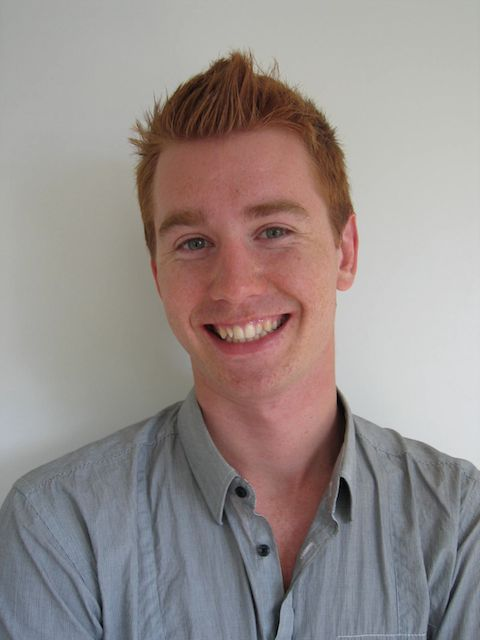
\includegraphics[width=2cm]{img/MHI.jpg} & Morten Hillebo (s072923)\tabularnewline
\end{tabular}
\par\end{center}
\end{document}


\begin{abstract}
 \begin{abstract}
This is the abstract.
\end{abstract}

\end{abstract}

\tableofcontents
\newpage

\section{Project description}
\label{sec:project_description}
The main requirements of the Vending Machine (VM):

\begin{enumerate}
\item The VM can sell one product, a coke-can.
\item When a sufficient amount of coins is inserted, one cocke-can will be dispensed from the VM.
\item The products price is fixed to 7 kr. ( in design this should be changeble )
\item The VM accepts 1 and 2 Kr coins.
\item A display should show the current total amount of money inserted.
\item A LED should indicate if change is avaliable (min 1 kr coin available).
\item Remove product sensor, will close the the coin slot and turn on indicating LED until product is removed.
\item Return Change.
\item Return all Coins.
\item If change is not available, the machine should only accept purchases with the right amount.
\end{enumerate}

 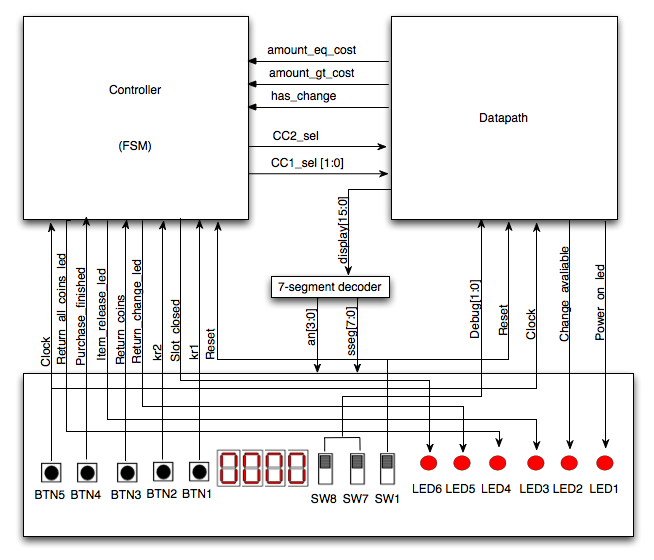
\includegraphics[scale=0.75]{fig/SystemDescription.png}


\section{Specification analysis}
The requirements on the processor dictates that a number of in- and output should be available. The values of these output is of course also to be respectively taken into account and verified.\\
By Studying the desciption of desired product, it quickly becomes apparent that our process has to implement and contain a number of states. We will also be needing numerous registers and other RTL level components.\\\\
First, we would need to (re)set currency and counter registers to an initial value. Having a register count up when a coin is inserted would make no sense unless reset at appopriate times. This leaves us with an init state.


\subsection{Requirements analysis}
By first doing a step-by-step analysis of the requirements, it becomes easier to implement every one of them in smaller steps.
\subsubsection*{Requirement 1}
The first requirement is that the machine should only be able to sell one type of product.\\
This is a requirement that actually simplifies the design, as it limits the user input we have to account for.

\subsubsection*{Requirement 2}
The machine dispenses one can at a time and dispenses as soon as the correct amount has been inserted.\\
This implies that we should do a transition to a dispense state if our amount is greater than or equal to the cost of one can.

\subsubsection*{Requirement 3}
The price must be changeable, though initially 7 kr.\\
By loading the cost into a register we could supply the cost via a bus. If the processor is implemented with an FPGA, it could also be specified in the VHDL code and then changed by rebuilding and reloading.

\subsubsection*{Requirement 4}
System accepts 1 and 2 Kr coins.\\
This can be implemented either by having a generic add state that does addition based on what coin was inserted, or by having separate states for adding 1 kr and adding 2 kr.

\subsubsection*{Requirement 5}
A display should show the total amount inserted.\\
This is solved by informal requirement described in section~\ref{sec:debug}. 

\subsubsection*{Requirement 6}
A LED should indicate if change is available.\\
In conjunction with requirement 4, this effectively becomes; the system should at least hold one 1 kr coin. 

\subsubsection*{Requirement 7}
The machine should close the coin slot until the product is removed. The original requirement is a bit ambiguous, as it state that the coin slot should be closed until the \emph{last} can has been removed. This contradicts requirement 1.\\
One way or the other, this gives us a wait state where we patiently wait for the user to remove the product.

\subsubsection*{Requirement 8}
The machine should be able to return change.\\
To detect if a user should receive change we need to able to detect if the amount of money inserted into the machine is more than cost of a product.

\subsubsection*{Requirement 9}
The user should at any time be able to cancel the purchase at any time up till the cost has been reached.\\


\subsubsection*{Requirement 10}
If change is not available, the machine should only accept purchases with the right amount.\\

\subsubsection*{Debug - informal requirement}
\label{sec:debug}

\section{Solution description}
\label{sec:solutions_description}
\paragraph{Req.1 One product, a coke-can.}
The cocke-can is the only product our vending machine can offer. This make the purchase senario of one coke-can our main senario. hence all our code revolves around this very requirement.

\paragraph{Req.2 When a sufficient amount is inserted, one cocke-can will be dispensed from the machine.} From the Purchase-state we will change to the Dispence-state if sufficient money has been inserted, that will lead to the dispence of one coke-can.

\begin{lstlisting}[caption={[VHDL]eks. text }]

\end{lstlisting}
  
\paragraph{Req.3 The product is fixed to 7 kr. ( in design this should be changeble ).} By changing this signal the price of one coke-can can can be changed. Unfortunately there are no inputs available for this action. we have agreed that a recompile would be neede to change the value. 
\begin{lstlisting}[caption={[VHDL]eks. text }]

\end{lstlisting}


\paragraph{Req.4 System accepts 1 and 2 Kr coins.}
lalala
\begin{lstlisting}[caption={[VHDL]eks. text }]

\end{lstlisting}
 

\paragraph{Req.5 A display should show the total amount inserted.}
lalala
\begin{lstlisting}[caption={[VHDL]eks. text }]

\end{lstlisting}
  

\paragraph{Req.6 A LED should indicate if change is avaliable (min 1 kr coin available).}
lalala
\begin{lstlisting}[caption={[VHDL]eks. text }]

\end{lstlisting}
 

\paragraph{Req.7 Remove product sensor, will close the the coin slot and turn on indicating LED until product is removed.}
lalala
\begin{lstlisting}[caption={[VHDL]eks. text }]

\end{lstlisting}  


\paragraph{Req.8 Return Change.}
lalala
\begin{lstlisting}[caption={[VHDL]eks. text }]

\end{lstlisting}
 

\paragraph{Req.9 Return Coins.}
lalala
\begin{lstlisting}[caption={[VHDL]eks. text }]

\end{lstlisting}


\paragraph{Req.10 If change is not available, the machine should only accept purchases with the right amount.}
lalala
\begin{lstlisting}[caption={[VHDL]eks. text }]

\end{lstlisting}



\section{Development process}
\label{sec:development_process}
A software development process is the structure needed to development any type of software products. 
There are several models for such development processes, each describing differed approaches to get the software developed.

\subsection{Software Development Models}
Many of the larger scale models such as Unified Process, Waterfall, Scrum or Spiral Model isn't suitable for small projects  of  4 weeks. But on the other hand Models like eXtreme Programming haven't got the diagrams and design phases needed for our learning curve of VHDL. The model we used was a mix of the differed models that had all the phases and methods we needed.

\subsection{Planning phase}
In this phase we read the assignment, analyze the requirements and go over the inputs, outputs and hints.
Then we made the first version of our High Level State Machine and.

\subsection{Implementation phase}
With the information from planning we started programming the VM. During this process we made our Data path diagram and several updates to the State Diagram.

\subsection{Testing phase}
In the Testing Phase all our test benches has been made to find the last few bugs and errors. 

\subsection{Documenting phase}
In the Documenting phase we had all the information needed. A working product, a lot of diagrams, and many test cases. We wrote our documentation in \LaTeXe  because it focuses more on documentation that typesetting and it makes managing and maintaining larger papers easier.	

\section{Tests}
\label{sec:tests}
During development of the circiut, we did out testing via a number of VHDL testbenches. These were used to assert that our 
develeopment went in the right direction, and also to verify that the indivudial circuits worked as planned.
\subsection{Testbenches}
During development we used three major testbenches. One for the combinatorial circuit, one for the register, and one for the 
two put together.



\section{Conclusion}
\chapter{Conclusion}
Writing up the business logic in both BEPL and REST has given a good insight in strengths and weaknesses of both technologies. While REST is, by far, the easiest technology to both get a working tool chain up and running for, and learning -- it is also the weakest in expressiveness.  BEPL, and hereby WDSL+SOAP provides an implicit documentation that is extremely valuable for project running for a very long time -- with many different developers -- as everything is described as business logic, or at least very close to native business logic as possible.\\\\
BEPL gives the best overview of the coordination between services -- and effectively also validation and verification thereof -- whereas REST relies on the ability of to write and understand code to, and general-purpose static analysis tools fed with the semantics of the model.

\newpage
\appendix
\section{Timetable}
\begin{center}
\begin{table}
\begin{tabular}{c|c|c|c|c|c|c|c}
Date & Individual & Design & Implementation & Test & Documentation & Other & Total\tabularnewline
\hline
\hline 
03/05/2010 & MHI & 6 &  &  &  &  & 6\tabularnewline
\hline 
03/05/2010 & KRC & 6 &  &  &  &  & 6\tabularnewline
\hline 
03/12/2010 & MHI &  & 4 &  &  &  & 4\tabularnewline
\hline 
03/12/2010 & KRC &  & 8 &  &  &  & 8\tabularnewline
\hline 
03/19/2010 & MHI &  &  & 6 &  &  & 6\tabularnewline
\hline 
03/19/2010 & KRC &  &  & 6 &  &  & 6\tabularnewline
\hline 
03/23/2010 & MHI &  &  &  & 8 &  & 8\tabularnewline
\hline 
03/23/2010 & KRC &  &  &  & 8 &  & 8\tabularnewline
\hline
\hline 
 & Total & 12 & 12 & 12 & 16 & 0 & 52\tabularnewline
\cline{2-8} 
\end{tabular}
\caption{Timetable \label{table:timetable} }
\end{table}
\end{center}

\section{Report distribution}
Kim Rostgaard Christensen (KRC)
\begin{itemize}
\item Sections \ref{sec:solutions_description} and \ref{sec:requirement_analysis}
\item Figures \ref{fig:fsm}, \ref{fig:fsmd}, \ref{fig:datapath} and \ref{fig:debug}
\end{itemize}

Morten Hillebo (MHI) 
\begin{itemize}
\item Sections \ref{sec:project_description}, \ref{sec:tests}
\end{itemize}


\section{Figures}
\label{app:figures}


\begin{figure}
\centering
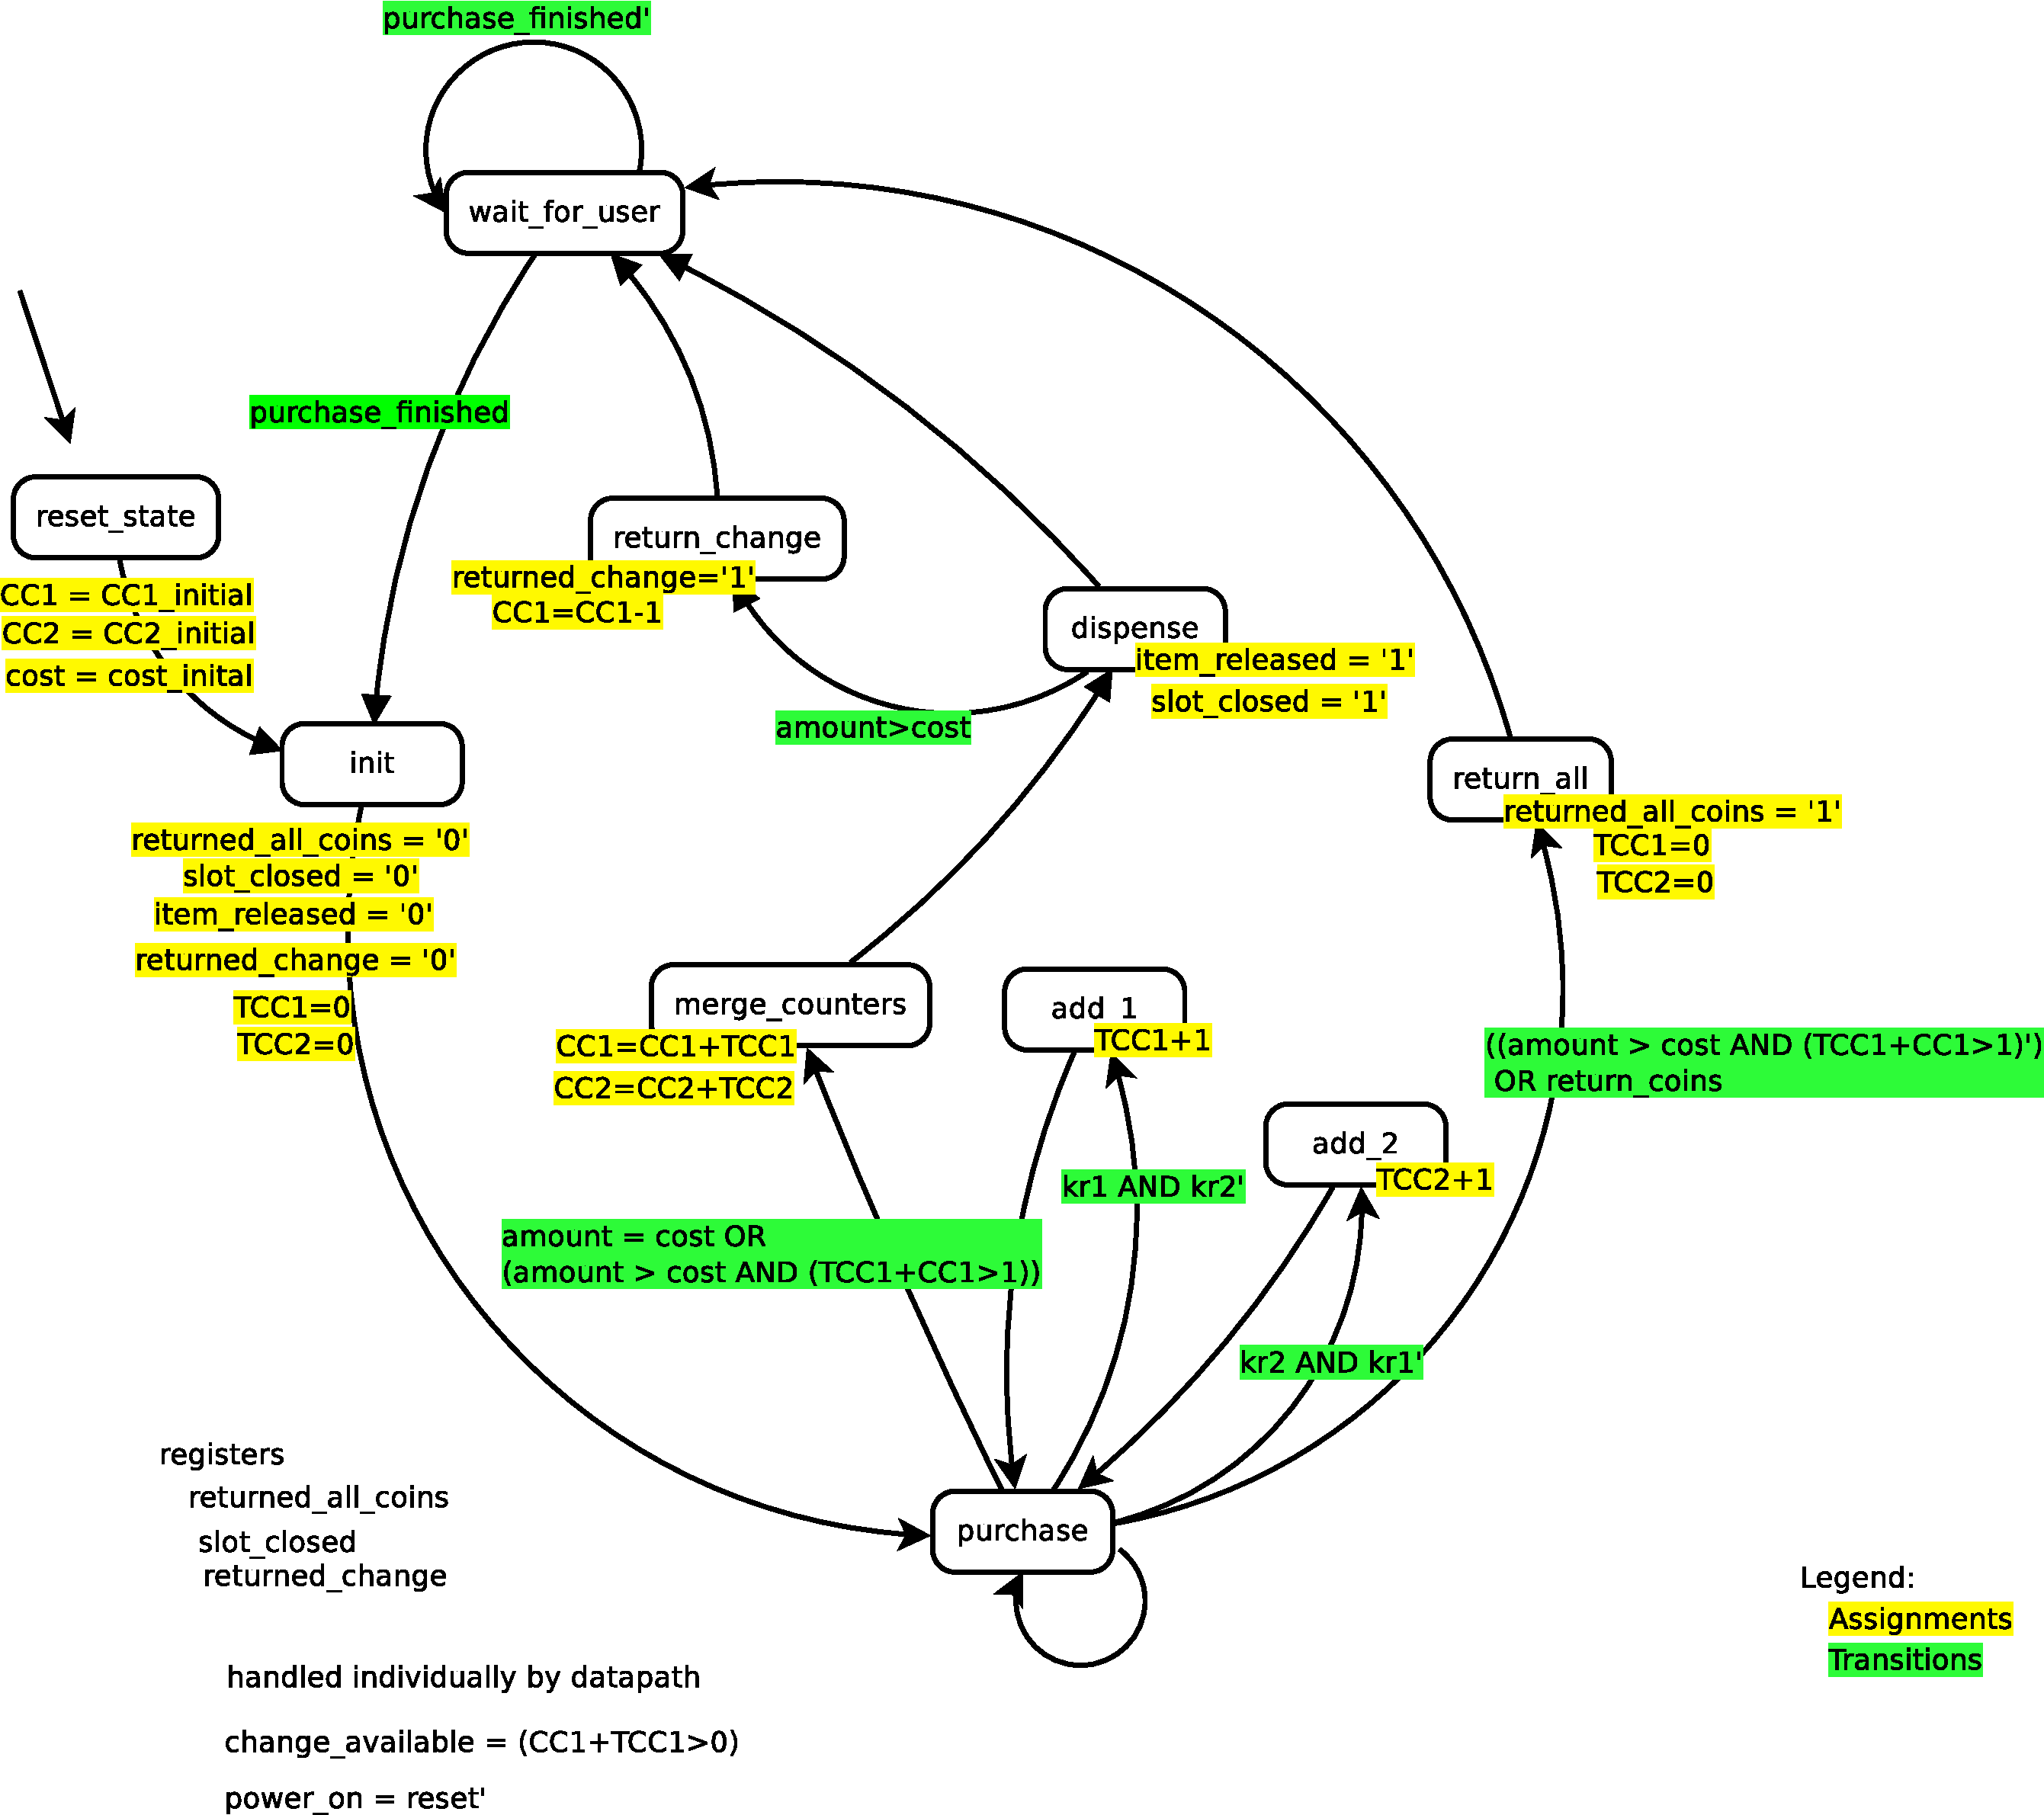
\includegraphics[width=1.0\textwidth]{fig/FSMD.pdf}
\caption{Finite statemachine with data}
\label{fig:fsmd}
\end{figure}

\begin{figure}
\centering
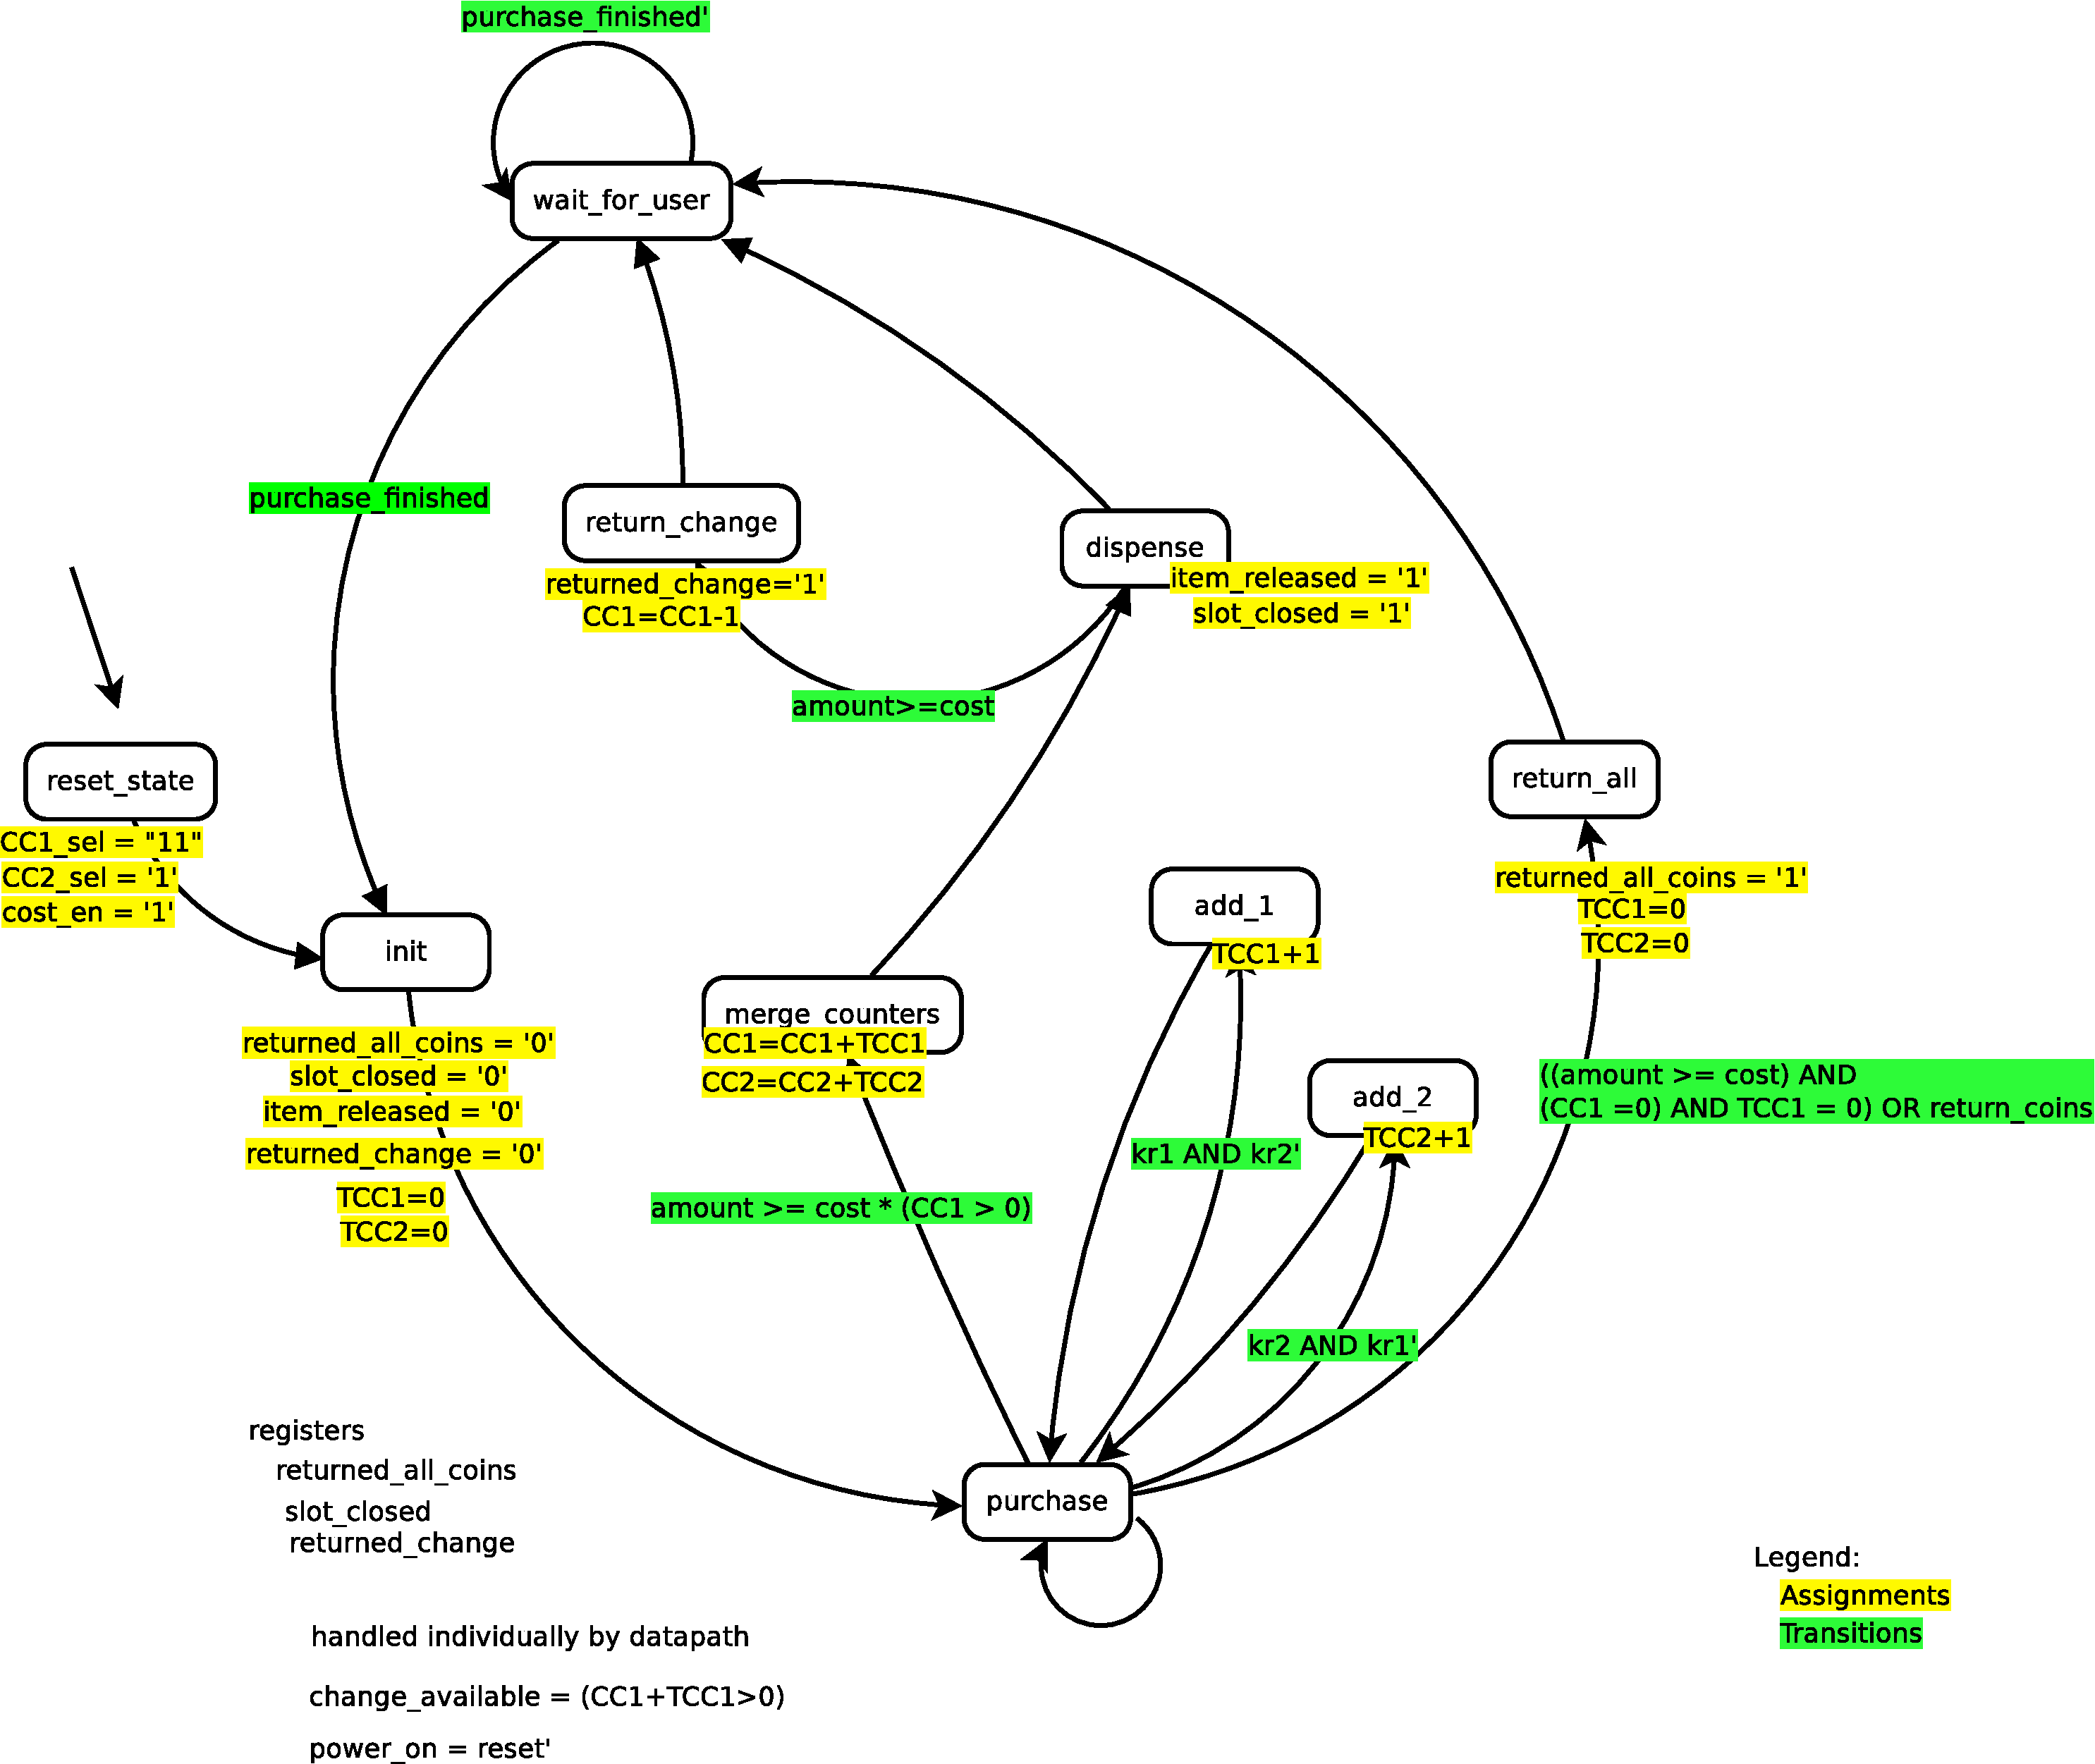
\includegraphics[width=1.0\textwidth]{fig/FSM.pdf}
\caption{Finite statemachine}
\label{fig:fsm}
\end{figure}

\begin{figure}
\centering
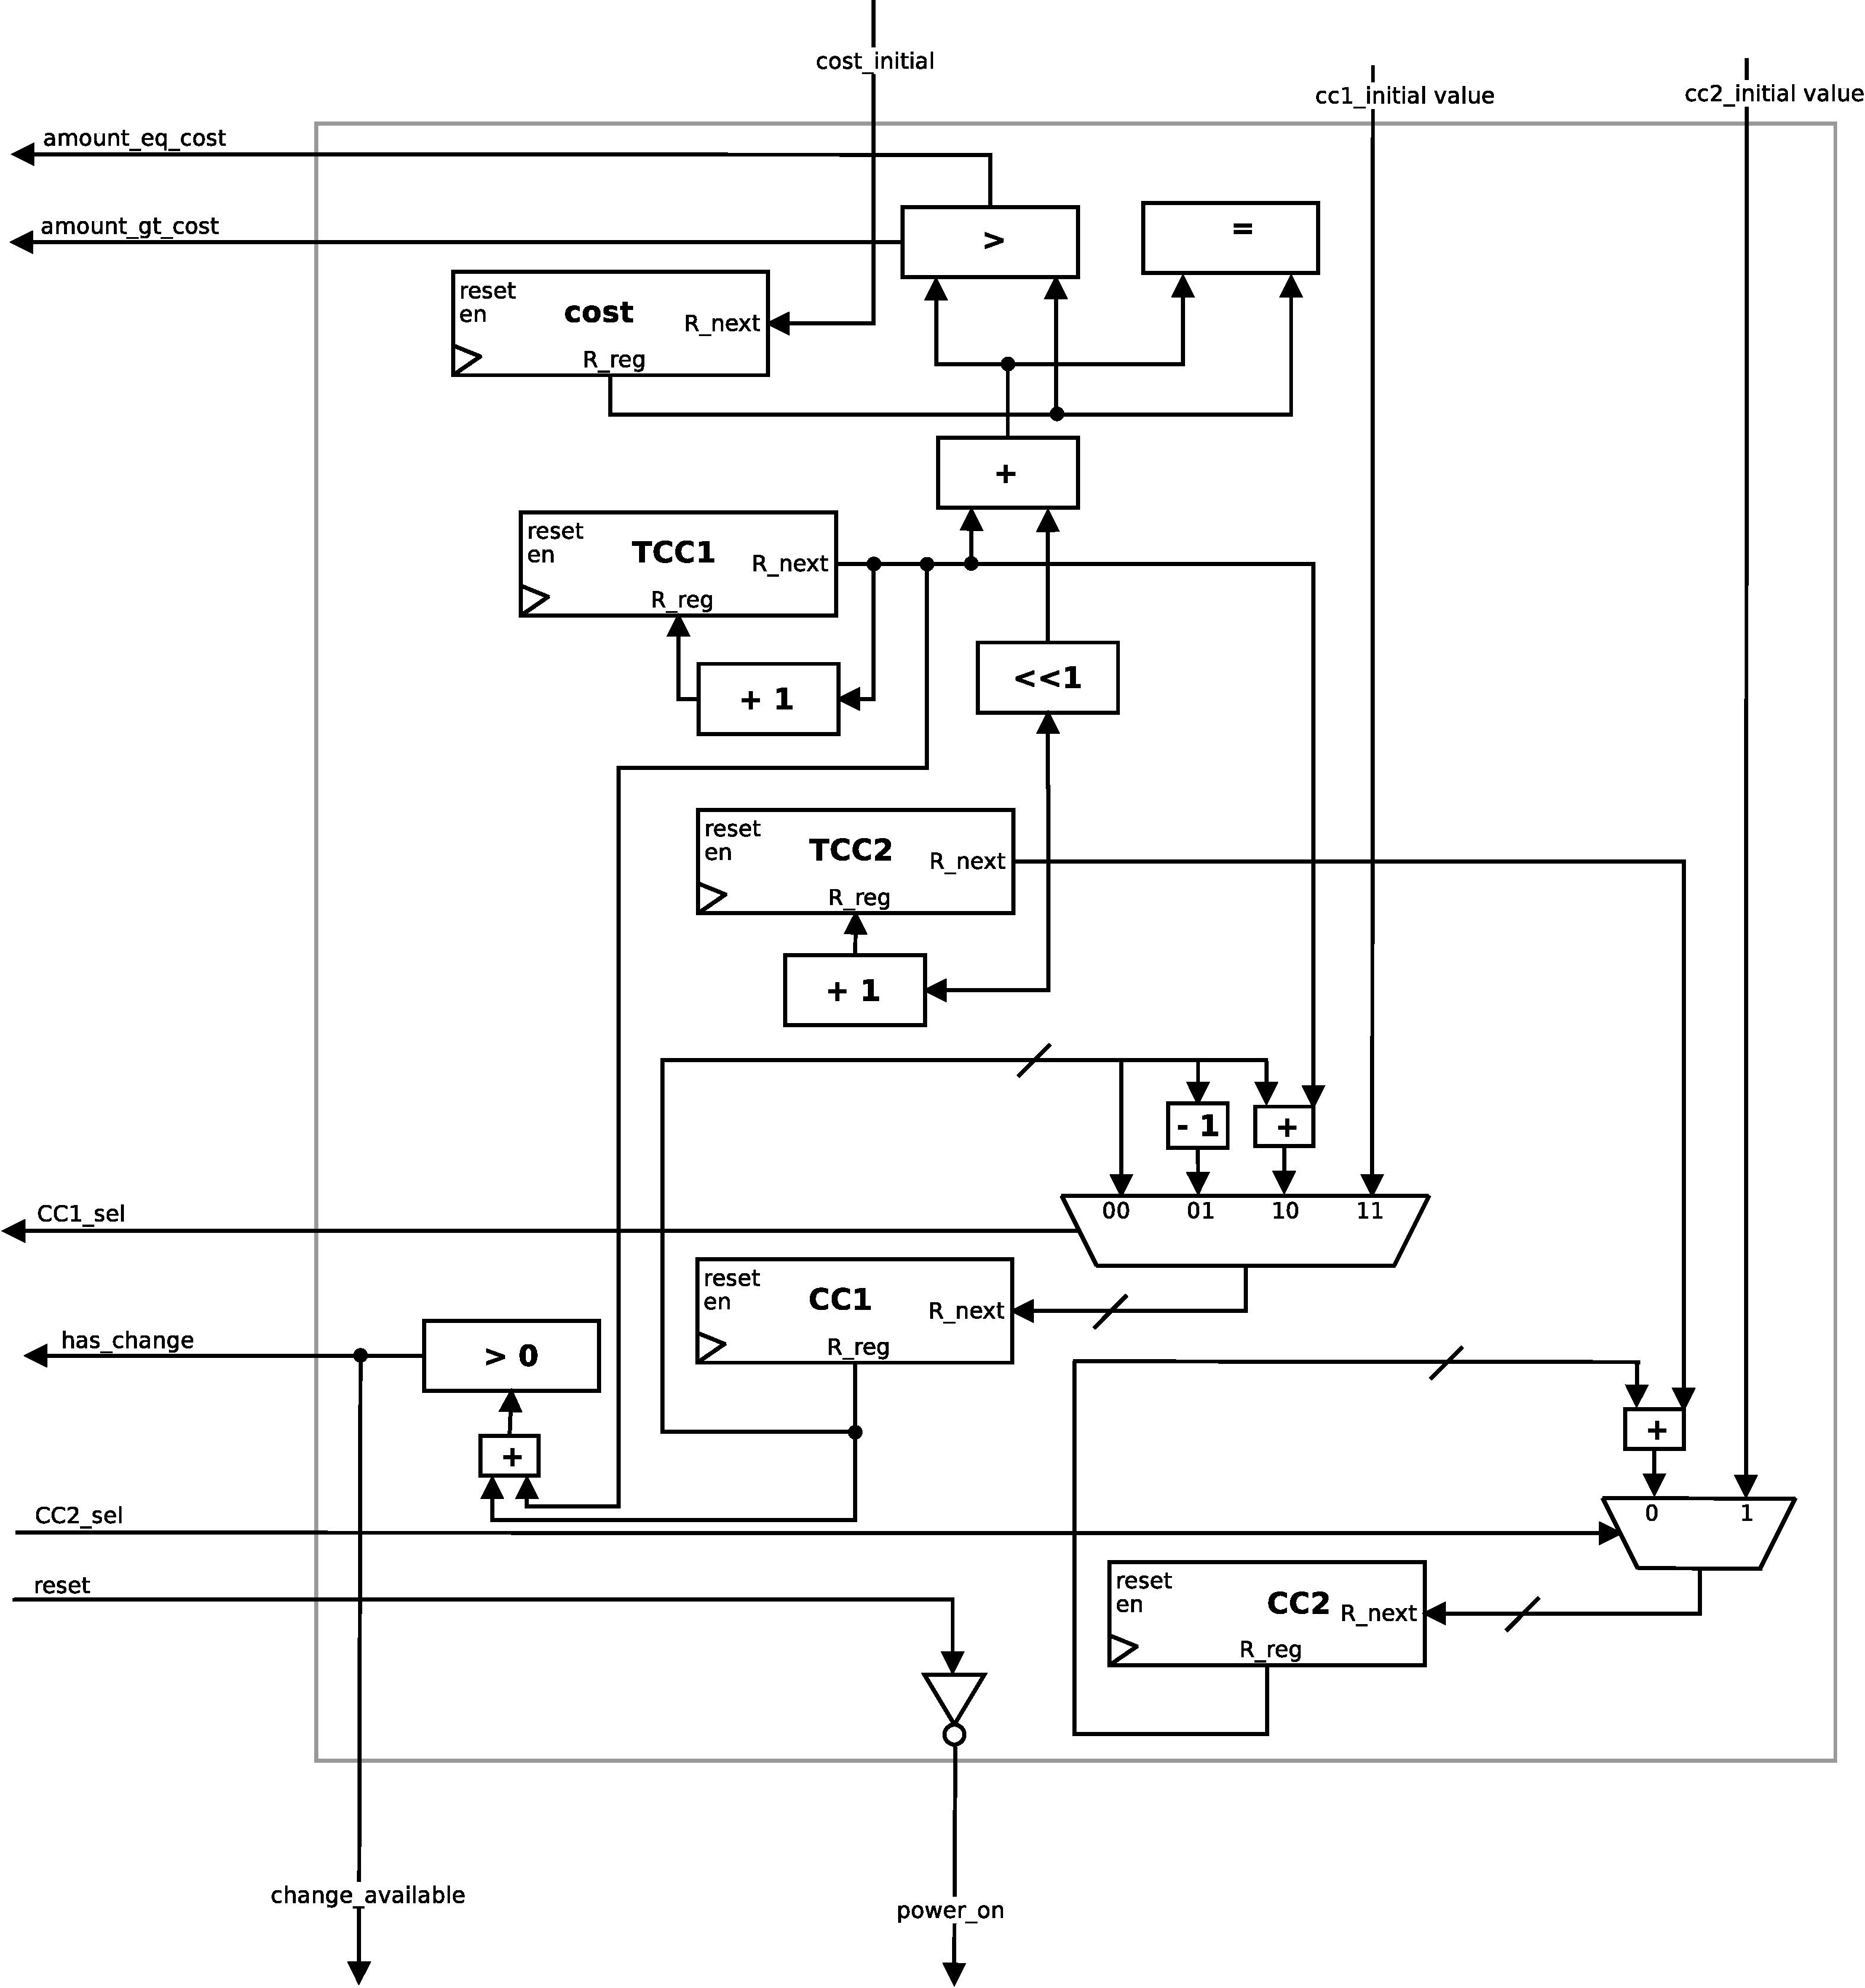
\includegraphics[width=1.0\textwidth]{fig/datapath.pdf}
\caption{Datapath of the processesor}
\label{fig:datapath}
\end{figure}

\begin{figure}
\centering
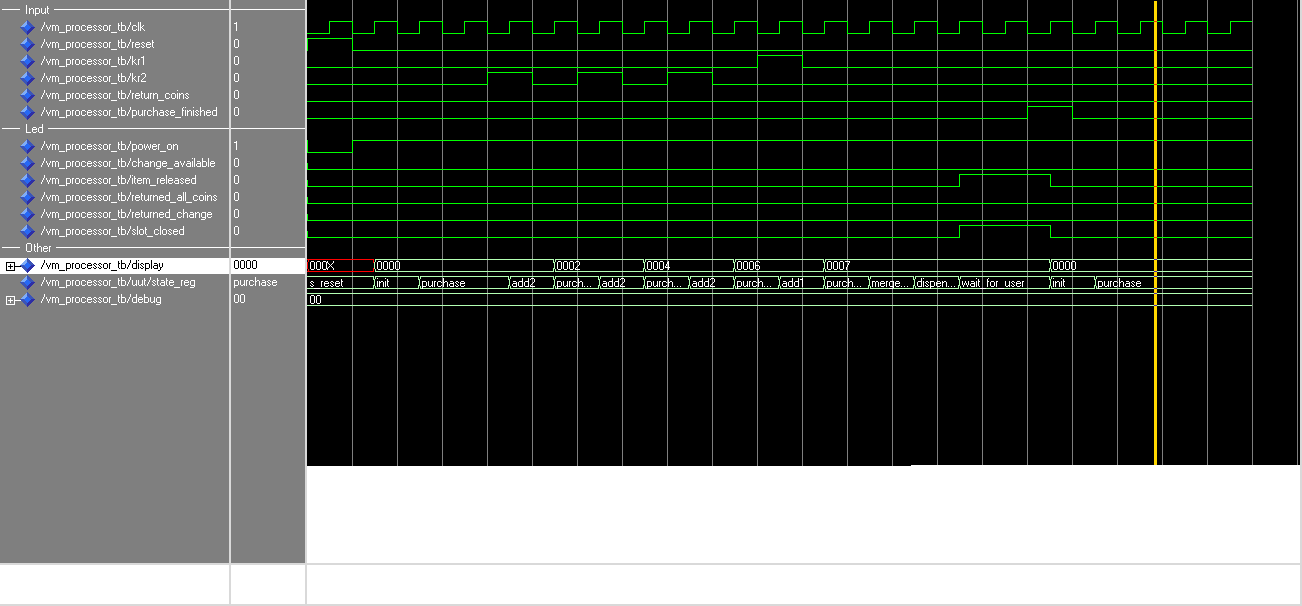
\includegraphics[width=0.6\textwidth]{img/wavetest1.png}
\caption{Test1 waveform}
\label{fig:test1}
\end{figure}

\begin{figure}
\centering
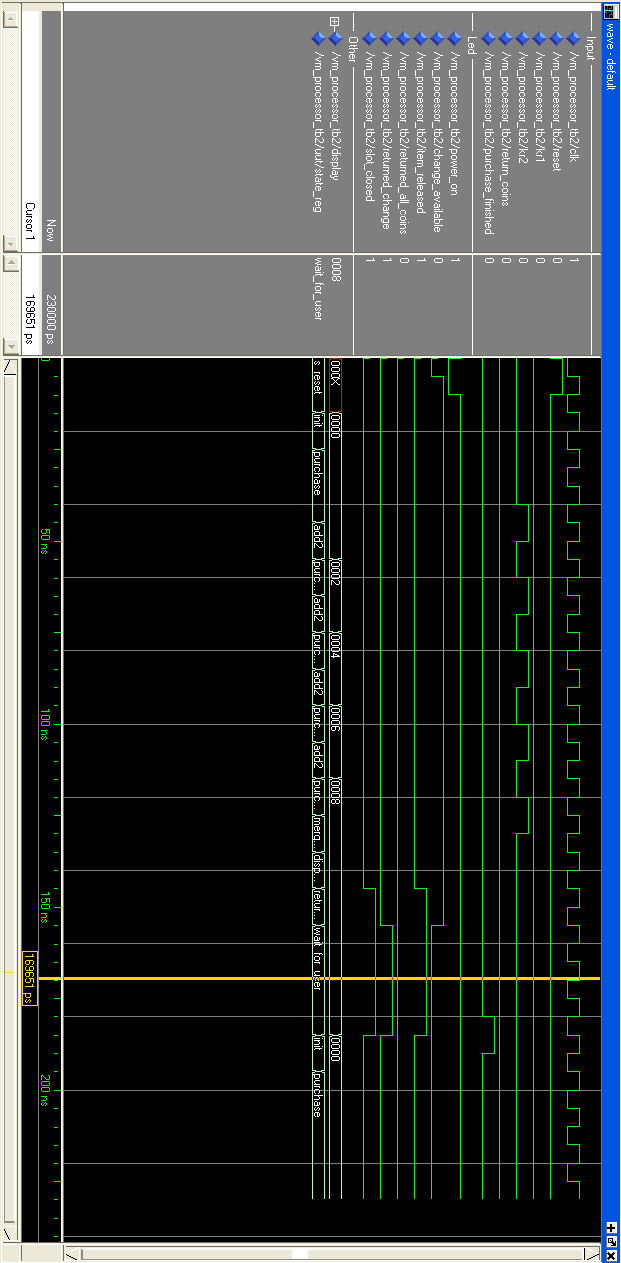
\includegraphics[width=0.6\textwidth]{img/wavetest2.png}
\caption{Test2 waveform}
\label{fig:test2}
\end{figure}

\begin{figure}
\centering
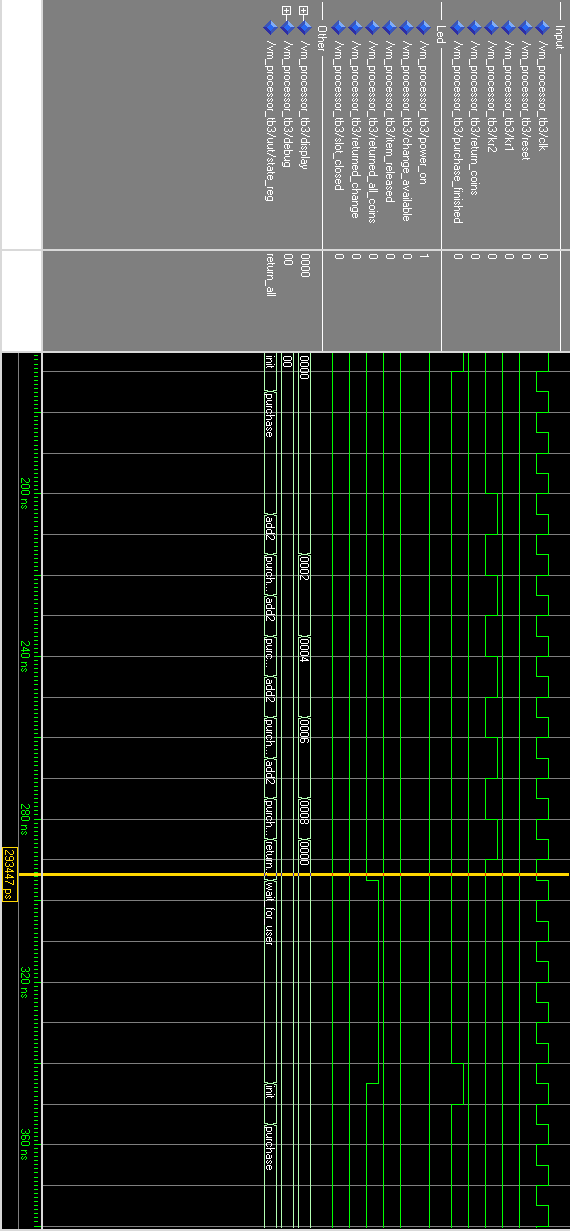
\includegraphics[width=0.6\textwidth]{img/wavetest3.png}
\caption{Test3 waveform}
\label{fig:test3}
\end{figure}

\begin{figure}
\centering
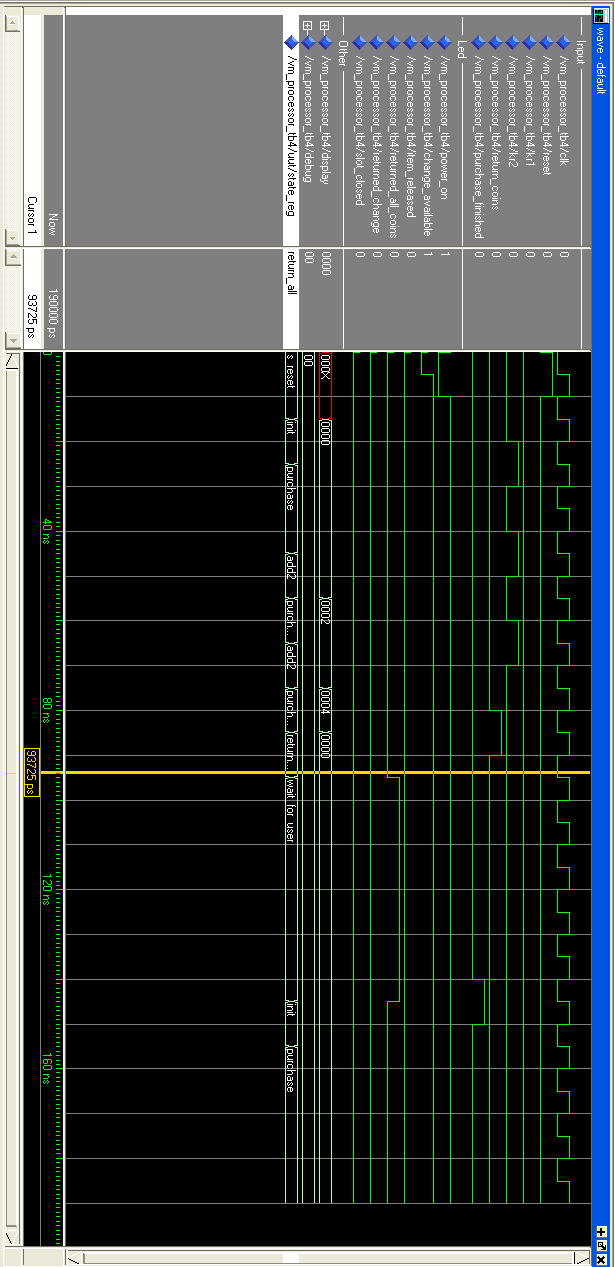
\includegraphics[width=0.6\textwidth]{img/wavetest4.png}
\caption{Test4 waveform}
\label{fig:test4}
\end{figure}

\begin{figure}
\centering
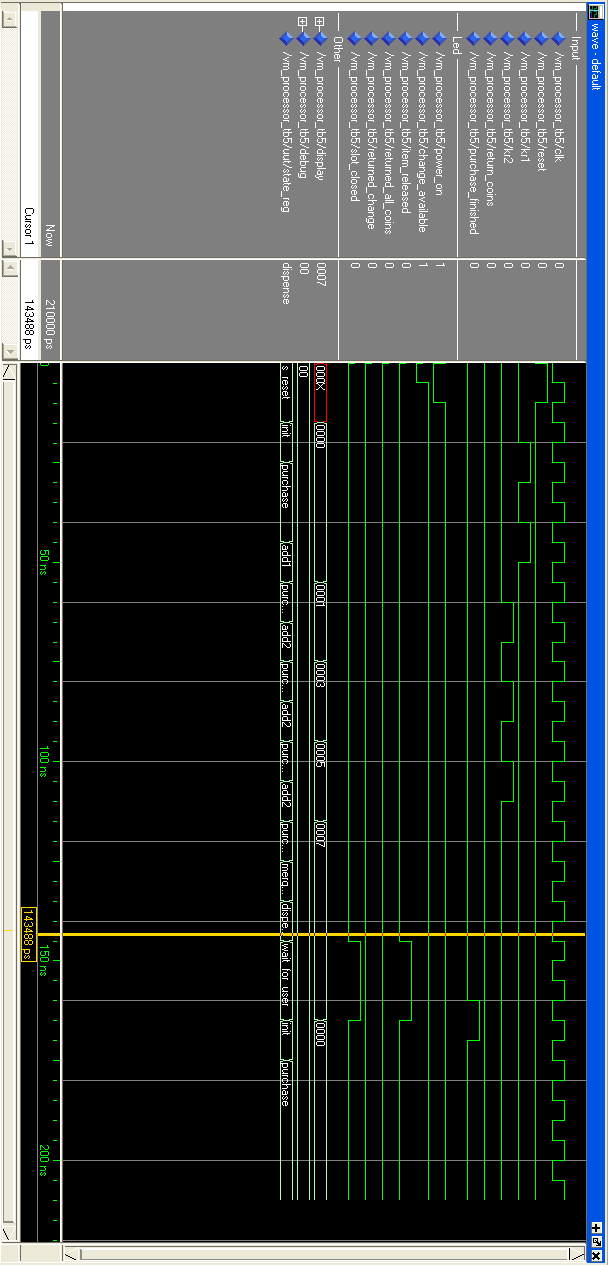
\includegraphics[width=0.6\textwidth]{img/wavetest5.png}
\caption{Test5 waveform}
\label{fig:test5}
\end{figure}

\end{document}
